% Options for packages loaded elsewhere
\PassOptionsToPackage{unicode}{hyperref}
\PassOptionsToPackage{hyphens}{url}
\PassOptionsToPackage{dvipsnames,svgnames,x11names}{xcolor}
%
\documentclass[
  11pt,
]{article}

\usepackage{amsmath,amssymb}
\usepackage{iftex}
\ifPDFTeX
  \usepackage[T1]{fontenc}
  \usepackage[utf8]{inputenc}
  \usepackage{textcomp} % provide euro and other symbols
\else % if luatex or xetex
  \usepackage{unicode-math}
  \defaultfontfeatures{Scale=MatchLowercase}
  \defaultfontfeatures[\rmfamily]{Ligatures=TeX,Scale=1}
\fi
\usepackage{lmodern}
\ifPDFTeX\else  
    % xetex/luatex font selection
\fi
% Use upquote if available, for straight quotes in verbatim environments
\IfFileExists{upquote.sty}{\usepackage{upquote}}{}
\IfFileExists{microtype.sty}{% use microtype if available
  \usepackage[]{microtype}
  \UseMicrotypeSet[protrusion]{basicmath} % disable protrusion for tt fonts
}{}
\makeatletter
\@ifundefined{KOMAClassName}{% if non-KOMA class
  \IfFileExists{parskip.sty}{%
    \usepackage{parskip}
  }{% else
    \setlength{\parindent}{0pt}
    \setlength{\parskip}{6pt plus 2pt minus 1pt}}
}{% if KOMA class
  \KOMAoptions{parskip=half}}
\makeatother
\usepackage{xcolor}
\usepackage[margin= 1in]{geometry}
\setlength{\emergencystretch}{3em} % prevent overfull lines
\setcounter{secnumdepth}{-\maxdimen} % remove section numbering
% Make \paragraph and \subparagraph free-standing
\ifx\paragraph\undefined\else
  \let\oldparagraph\paragraph
  \renewcommand{\paragraph}[1]{\oldparagraph{#1}\mbox{}}
\fi
\ifx\subparagraph\undefined\else
  \let\oldsubparagraph\subparagraph
  \renewcommand{\subparagraph}[1]{\oldsubparagraph{#1}\mbox{}}
\fi

\usepackage{color}
\usepackage{fancyvrb}
\newcommand{\VerbBar}{|}
\newcommand{\VERB}{\Verb[commandchars=\\\{\}]}
\DefineVerbatimEnvironment{Highlighting}{Verbatim}{commandchars=\\\{\}}
% Add ',fontsize=\small' for more characters per line
\usepackage{framed}
\definecolor{shadecolor}{RGB}{241,243,245}
\newenvironment{Shaded}{\begin{snugshade}}{\end{snugshade}}
\newcommand{\AlertTok}[1]{\textcolor[rgb]{0.68,0.00,0.00}{#1}}
\newcommand{\AnnotationTok}[1]{\textcolor[rgb]{0.37,0.37,0.37}{#1}}
\newcommand{\AttributeTok}[1]{\textcolor[rgb]{0.40,0.45,0.13}{#1}}
\newcommand{\BaseNTok}[1]{\textcolor[rgb]{0.68,0.00,0.00}{#1}}
\newcommand{\BuiltInTok}[1]{\textcolor[rgb]{0.00,0.23,0.31}{#1}}
\newcommand{\CharTok}[1]{\textcolor[rgb]{0.13,0.47,0.30}{#1}}
\newcommand{\CommentTok}[1]{\textcolor[rgb]{0.37,0.37,0.37}{#1}}
\newcommand{\CommentVarTok}[1]{\textcolor[rgb]{0.37,0.37,0.37}{\textit{#1}}}
\newcommand{\ConstantTok}[1]{\textcolor[rgb]{0.56,0.35,0.01}{#1}}
\newcommand{\ControlFlowTok}[1]{\textcolor[rgb]{0.00,0.23,0.31}{#1}}
\newcommand{\DataTypeTok}[1]{\textcolor[rgb]{0.68,0.00,0.00}{#1}}
\newcommand{\DecValTok}[1]{\textcolor[rgb]{0.68,0.00,0.00}{#1}}
\newcommand{\DocumentationTok}[1]{\textcolor[rgb]{0.37,0.37,0.37}{\textit{#1}}}
\newcommand{\ErrorTok}[1]{\textcolor[rgb]{0.68,0.00,0.00}{#1}}
\newcommand{\ExtensionTok}[1]{\textcolor[rgb]{0.00,0.23,0.31}{#1}}
\newcommand{\FloatTok}[1]{\textcolor[rgb]{0.68,0.00,0.00}{#1}}
\newcommand{\FunctionTok}[1]{\textcolor[rgb]{0.28,0.35,0.67}{#1}}
\newcommand{\ImportTok}[1]{\textcolor[rgb]{0.00,0.46,0.62}{#1}}
\newcommand{\InformationTok}[1]{\textcolor[rgb]{0.37,0.37,0.37}{#1}}
\newcommand{\KeywordTok}[1]{\textcolor[rgb]{0.00,0.23,0.31}{#1}}
\newcommand{\NormalTok}[1]{\textcolor[rgb]{0.00,0.23,0.31}{#1}}
\newcommand{\OperatorTok}[1]{\textcolor[rgb]{0.37,0.37,0.37}{#1}}
\newcommand{\OtherTok}[1]{\textcolor[rgb]{0.00,0.23,0.31}{#1}}
\newcommand{\PreprocessorTok}[1]{\textcolor[rgb]{0.68,0.00,0.00}{#1}}
\newcommand{\RegionMarkerTok}[1]{\textcolor[rgb]{0.00,0.23,0.31}{#1}}
\newcommand{\SpecialCharTok}[1]{\textcolor[rgb]{0.37,0.37,0.37}{#1}}
\newcommand{\SpecialStringTok}[1]{\textcolor[rgb]{0.13,0.47,0.30}{#1}}
\newcommand{\StringTok}[1]{\textcolor[rgb]{0.13,0.47,0.30}{#1}}
\newcommand{\VariableTok}[1]{\textcolor[rgb]{0.07,0.07,0.07}{#1}}
\newcommand{\VerbatimStringTok}[1]{\textcolor[rgb]{0.13,0.47,0.30}{#1}}
\newcommand{\WarningTok}[1]{\textcolor[rgb]{0.37,0.37,0.37}{\textit{#1}}}

\providecommand{\tightlist}{%
  \setlength{\itemsep}{0pt}\setlength{\parskip}{0pt}}\usepackage{longtable,booktabs,array}
\usepackage{calc} % for calculating minipage widths
% Correct order of tables after \paragraph or \subparagraph
\usepackage{etoolbox}
\makeatletter
\patchcmd\longtable{\par}{\if@noskipsec\mbox{}\fi\par}{}{}
\makeatother
% Allow footnotes in longtable head/foot
\IfFileExists{footnotehyper.sty}{\usepackage{footnotehyper}}{\usepackage{footnote}}
\makesavenoteenv{longtable}
\usepackage{graphicx}
\makeatletter
\def\maxwidth{\ifdim\Gin@nat@width>\linewidth\linewidth\else\Gin@nat@width\fi}
\def\maxheight{\ifdim\Gin@nat@height>\textheight\textheight\else\Gin@nat@height\fi}
\makeatother
% Scale images if necessary, so that they will not overflow the page
% margins by default, and it is still possible to overwrite the defaults
% using explicit options in \includegraphics[width, height, ...]{}
\setkeys{Gin}{width=\maxwidth,height=\maxheight,keepaspectratio}
% Set default figure placement to htbp
\makeatletter
\def\fps@figure{htbp}
\makeatother

\usepackage{fvextra}
\DefineVerbatimEnvironment{Highlighting}{Verbatim}{breaklines,commandchars=\\\{\}}
\DefineVerbatimEnvironment{OutputCode}{Verbatim}{breaklines,commandchars=\\\{\}}
\fvset{breaksymbolleft={}, breakindent=1em}
\makeatletter
\@ifpackageloaded{caption}{}{\usepackage{caption}}
\AtBeginDocument{%
\ifdefined\contentsname
  \renewcommand*\contentsname{Table of contents}
\else
  \newcommand\contentsname{Table of contents}
\fi
\ifdefined\listfigurename
  \renewcommand*\listfigurename{List of Figures}
\else
  \newcommand\listfigurename{List of Figures}
\fi
\ifdefined\listtablename
  \renewcommand*\listtablename{List of Tables}
\else
  \newcommand\listtablename{List of Tables}
\fi
\ifdefined\figurename
  \renewcommand*\figurename{Figure}
\else
  \newcommand\figurename{Figure}
\fi
\ifdefined\tablename
  \renewcommand*\tablename{Table}
\else
  \newcommand\tablename{Table}
\fi
}
\@ifpackageloaded{float}{}{\usepackage{float}}
\floatstyle{ruled}
\@ifundefined{c@chapter}{\newfloat{codelisting}{h}{lop}}{\newfloat{codelisting}{h}{lop}[chapter]}
\floatname{codelisting}{Listing}
\newcommand*\listoflistings{\listof{codelisting}{List of Listings}}
\makeatother
\makeatletter
\makeatother
\makeatletter
\@ifpackageloaded{caption}{}{\usepackage{caption}}
\@ifpackageloaded{subcaption}{}{\usepackage{subcaption}}
\makeatother
\ifLuaTeX
  \usepackage{selnolig}  % disable illegal ligatures
\fi
\usepackage{bookmark}

\IfFileExists{xurl.sty}{\usepackage{xurl}}{} % add URL line breaks if available
\urlstyle{same} % disable monospaced font for URLs
\hypersetup{
  pdftitle={Homework 5},
  pdfauthor={Nick Climaco},
  colorlinks=true,
  linkcolor={blue},
  filecolor={Maroon},
  citecolor={Blue},
  urlcolor={Blue},
  pdfcreator={LaTeX via pandoc}}

\title{Homework 5}
\author{Nick Climaco}
\date{March 3, 2024}

\begin{document}
\maketitle

\renewcommand*\contentsname{Table of contents}
{
\hypersetup{linkcolor=}
\setcounter{tocdepth}{3}
\tableofcontents
}
\section{HA Chapter 8: Exponential
Smoothing}\label{ha-chapter-8-exponential-smoothing}

\#\textbar{} message : false

\#\textbar{} output : false

\subsection{import libraries}\label{import-libraries}

\begin{center}\rule{0.5\linewidth}{0.5pt}\end{center}

\subsection{Exercise 8.1}\label{exercise-8.1}

Consider the the number of pigs slaughtered in Victoria, available in
the aus\_livestock dataset.

\begin{longtable}[]{@{}lllll@{}}
\toprule\noalign{}
& Unnamed: 0 & Animal & State & Count \\
Month & & & & \\
\midrule\noalign{}
\endhead
\bottomrule\noalign{}
\endlastfoot
1976-07-01 & 1 & Bulls, bullocks and steers & Australian Capital
Territory & 2300.0 \\
1976-08-01 & 2 & Bulls, bullocks and steers & Australian Capital
Territory & 2100.0 \\
1976-09-01 & 3 & Bulls, bullocks and steers & Australian Capital
Territory & 2100.0 \\
1976-10-01 & 4 & Bulls, bullocks and steers & Australian Capital
Territory & 1900.0 \\
1976-11-01 & 5 & Bulls, bullocks and steers & Australian Capital
Territory & 2100.0 \\
... & ... & ... & ... & ... \\
2018-08-01 & 29360 & Sheep & Western Australia & 160600.0 \\
2018-09-01 & 29361 & Sheep & Western Australia & 121900.0 \\
2018-10-01 & 29362 & Sheep & Western Australia & 134000.0 \\
2018-11-01 & 29363 & Sheep & Western Australia & 153700.0 \\
2018-12-01 & 29364 & Sheep & Western Australia & 127300.0 \\
\end{longtable}

\subsubsection{Part A}\label{part-a}

Use the ETS() function to estimate the equivalent model for simple
exponential smoothing. Find the optimal values of α and \(ℓ_0\), and
generate forecasts for the next four months.

\begin{Shaded}
\begin{Highlighting}[]
\CommentTok{\# filter data}
\NormalTok{victorian\_pigs }\OperatorTok{=}\NormalTok{ aus\_livestock.query(}\StringTok{\textquotesingle{}Animal == "Pigs" \& State == "Victoria"\textquotesingle{}}\NormalTok{)[[}\StringTok{\textquotesingle{}Count\textquotesingle{}}\NormalTok{]]}
\end{Highlighting}
\end{Shaded}

\begin{Shaded}
\begin{Highlighting}[]
\ImportTok{from}\NormalTok{ statsmodels.tsa.holtwinters }\ImportTok{import}\NormalTok{ ExponentialSmoothing}

\NormalTok{model }\OperatorTok{=}\NormalTok{ ExponentialSmoothing(victorian\_pigs, trend }\OperatorTok{=} \StringTok{\textquotesingle{}additive\textquotesingle{}}\NormalTok{, seasonal }\OperatorTok{=} \VariableTok{None}\NormalTok{).fit()}

\NormalTok{predictions }\OperatorTok{=}\NormalTok{ model.forecast(steps}\OperatorTok{=}\DecValTok{4}\NormalTok{) }\CommentTok{\# predict the next 4 time steps}
\end{Highlighting}
\end{Shaded}

\begin{Shaded}
\begin{Highlighting}[]
\NormalTok{victorian\_pigs.tail()}
\end{Highlighting}
\end{Shaded}

\begin{longtable}[]{@{}ll@{}}
\toprule\noalign{}
& Count \\
Month & \\
\midrule\noalign{}
\endhead
\bottomrule\noalign{}
\endlastfoot
2018-08-01 & 102500.0 \\
2018-09-01 & 82600.0 \\
2018-10-01 & 100700.0 \\
2018-11-01 & 98500.0 \\
2018-12-01 & 92300.0 \\
\end{longtable}

\begin{Shaded}
\begin{Highlighting}[]
\BuiltInTok{print}\NormalTok{(model.summary())}
\end{Highlighting}
\end{Shaded}

\begin{verbatim}
                       ExponentialSmoothing Model Results                       
================================================================================
Dep. Variable:                    Count   No. Observations:                  558
Model:             ExponentialSmoothing   SSE                    49759385612.180
Optimized:                         True   AIC                          10222.807
Trend:                         Additive   BIC                          10240.105
Seasonal:                          None   AICC                         10222.960
Seasonal Periods:                  None   Date:                 Sun, 03 Mar 2024
Box-Cox:                          False   Time:                         18:57:44
Box-Cox Coeff.:                    None                                         
==============================================================================
                       coeff                 code              optimized      
------------------------------------------------------------------------------
smoothing_level            0.3350000                alpha                 True
smoothing_trend            0.0279167                 beta                 True
initial_level             1.0843e+05                  l.0                 True
initial_trend             -1924.8485                  b.0                 True
------------------------------------------------------------------------------
\end{verbatim}

The optimal \(\alpha = 0.335\) and \(l_0 =  1.0843e+05\).

Having a lower alpha estimates means that the exponential decay is
slower and we can expected that the next 4 forecasts will be close in
value.

The forecasts for the next 4 time steps are below.

\begin{Shaded}
\begin{Highlighting}[]
\BuiltInTok{print}\NormalTok{(predictions)}
\end{Highlighting}
\end{Shaded}

\begin{verbatim}
2019-01-01    95532.225056
2019-02-01    95637.681211
2019-03-01    95743.137366
2019-04-01    95848.593521
Freq: MS, dtype: float64
\end{verbatim}

\subsubsection{Part B}\label{part-b}

Compute a 95\% prediction interval for the first forecast using
\(\hat{y}±1.96s\) where \(s\) is the standard deviation of the
residuals. Compare your interval with the interval produced by R

\begin{Shaded}
\begin{Highlighting}[]
\CommentTok{\# we need to calc only the first forecast }
\NormalTok{residuals\_std }\OperatorTok{=}\NormalTok{ model.resid.std()}

\NormalTok{first\_forecast }\OperatorTok{=}\NormalTok{ predictions.iloc[}\DecValTok{0}\NormalTok{]}

\NormalTok{margin\_of\_error }\OperatorTok{=} \FloatTok{1.96} \OperatorTok{*}\NormalTok{ residuals\_std}

\NormalTok{lower\_limit }\OperatorTok{=}\NormalTok{ first\_forecast }\OperatorTok{{-}}\NormalTok{ margin\_of\_error}
\NormalTok{upper\_limit }\OperatorTok{=}\NormalTok{ first\_forecast }\OperatorTok{+}\NormalTok{ margin\_of\_error}

\BuiltInTok{print}\NormalTok{(}\SpecialStringTok{f\textquotesingle{}95\% Prediction Interval: (}\SpecialCharTok{\{}\NormalTok{lower\_limit}\SpecialCharTok{:.2f\}}\SpecialStringTok{, }\SpecialCharTok{\{}\NormalTok{upper\_limit}\SpecialCharTok{:.2f\}}\SpecialStringTok{)\textquotesingle{}}\NormalTok{)}
\end{Highlighting}
\end{Shaded}

\begin{verbatim}
95% Prediction Interval: (77022.62, 114041.83)
\end{verbatim}

Rcode :

\begin{Shaded}
\begin{Highlighting}[]

\NormalTok{\textasciigrave{}\textasciigrave{}\textasciigrave{}\{r\}}
\NormalTok{fc |\textgreater{}}
\NormalTok{  autoplot(tail(vic\_pigs, 5)) +}
\NormalTok{  geom\_line(aes(y = .fitted), col="\#D55E00",}
\NormalTok{            data = augment(fit)) +}
\NormalTok{  labs(y="\% of GDP", title="Victorian Pigs") +}
\NormalTok{  guides(colour = "none")}
\end{Highlighting}
\end{Shaded}

` ` `

\begin{figure}[H]

{\centering 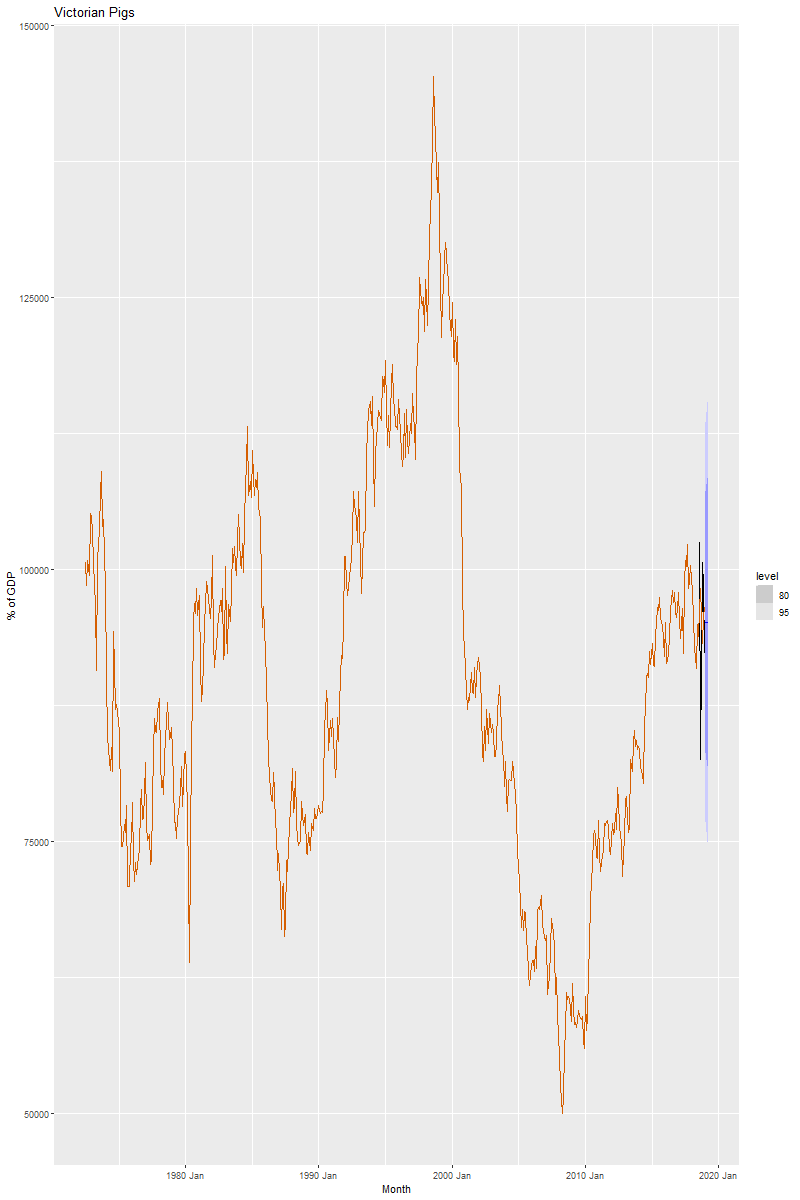
\includegraphics{hw5_files/figure-pdf/cell-20-1-image.png}

}

\caption{image.png}

\end{figure}%

My 95\% confidence intervals is narrower compared to the confidence
interval produced from the Rcode. We suspect that this may due to
different smoothing and leveling estimates.

\begin{center}\rule{0.5\linewidth}{0.5pt}\end{center}

\subsection{Exercise 8.5}\label{exercise-8.5}

Data set \texttt{global\_economy} contains the annual Exports from many
countries. Select one country to analyse.

\subsubsection{Part A}\label{part-a-1}

Plot the Exports series and discuss the main features of the data

\begin{Shaded}
\begin{Highlighting}[]
\NormalTok{canada\_exports }\OperatorTok{=}\NormalTok{ global\_economy.query(}\StringTok{\textquotesingle{}Country == "Canada"\textquotesingle{}}\NormalTok{)[[}\StringTok{\textquotesingle{}Exports\textquotesingle{}}\NormalTok{]]}
\end{Highlighting}
\end{Shaded}

\begin{Shaded}
\begin{Highlighting}[]
\NormalTok{canada\_exports.plot()}
\NormalTok{plt.title(}\StringTok{\textquotesingle{}Canadian Exports\textquotesingle{}}\NormalTok{)}
\NormalTok{plt.show()}
\end{Highlighting}
\end{Shaded}

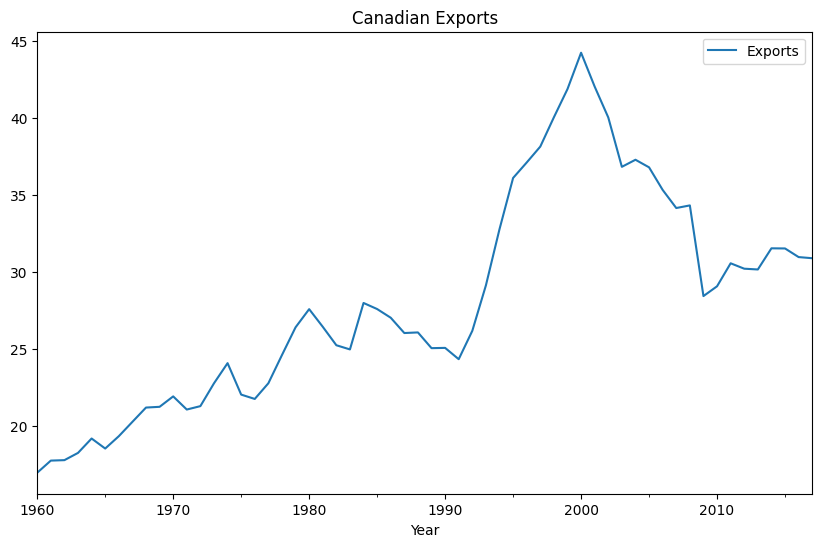
\includegraphics{hw5_files/figure-pdf/cell-13-output-1.png}

\begin{Shaded}
\begin{Highlighting}[]
\ImportTok{from}\NormalTok{ statsmodels.tsa.seasonal }\ImportTok{import}\NormalTok{ seasonal\_decompose}

\NormalTok{result }\OperatorTok{=}\NormalTok{ seasonal\_decompose(canada\_exports, model}\OperatorTok{=}\StringTok{\textquotesingle{}additive\textquotesingle{}}\NormalTok{)}
\NormalTok{result.plot()}
\NormalTok{plt.show()}
\end{Highlighting}
\end{Shaded}

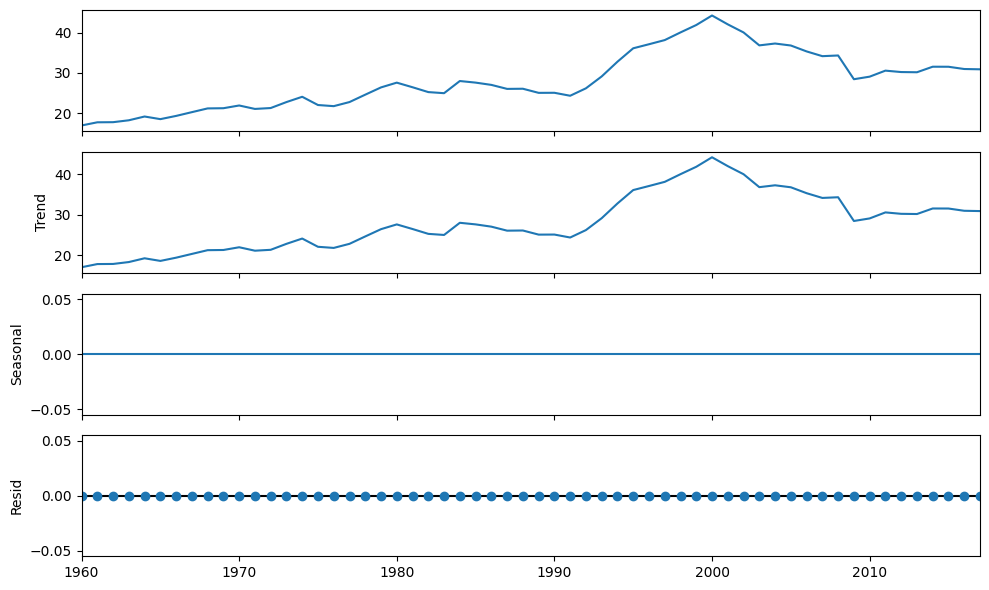
\includegraphics{hw5_files/figure-pdf/cell-14-output-1.png}

Canada's exports exhibits a overall upward trend from 1960 to 2017, with
a notable growth during the 1990s. This trend peaked around the year
2000, followed by a decline until 2010 where it started to stabilize.
The time series decomposition confirms the absence of seasonality,
demosntrating a straight line seasonal component.

\subsubsection{Part B}\label{part-b-1}

Use an ETS(A,N,N) model to forecast the series, and plot the forecasts.

\begin{Shaded}
\begin{Highlighting}[]
\CommentTok{\# train test split }
\NormalTok{train\_data, test\_data }\OperatorTok{=}\NormalTok{ canada\_exports[}\DecValTok{0}\NormalTok{:}\BuiltInTok{int}\NormalTok{(}\BuiltInTok{len}\NormalTok{(canada\_exports)}\OperatorTok{*}\FloatTok{0.8}\NormalTok{)], canada\_exports[}\BuiltInTok{int}\NormalTok{(}\BuiltInTok{len}\NormalTok{(canada\_exports)}\OperatorTok{*}\FloatTok{0.8}\NormalTok{):]}
\end{Highlighting}
\end{Shaded}

\begin{Shaded}
\begin{Highlighting}[]
\CommentTok{\# ETS(A,N,N) would be trend = \textquotesingle{}add\textquotesingle{} and damped\_trend = False}
\ImportTok{from}\NormalTok{ statsmodels.tsa.exponential\_smoothing.ets }\ImportTok{import}\NormalTok{ ETSModel}

\NormalTok{ets\_model }\OperatorTok{=}\NormalTok{ ETSModel(train\_data[}\StringTok{\textquotesingle{}Exports\textquotesingle{}}\NormalTok{], trend }\OperatorTok{=} \StringTok{\textquotesingle{}add\textquotesingle{}}\NormalTok{, damped\_trend }\OperatorTok{=} \VariableTok{False}\NormalTok{, seasonal }\OperatorTok{=} \VariableTok{None}\NormalTok{).fit()}

\NormalTok{forecast }\OperatorTok{=}\NormalTok{ ets\_model.forecast(steps}\OperatorTok{=}\BuiltInTok{len}\NormalTok{(test\_data))}
\end{Highlighting}
\end{Shaded}

\begin{verbatim}
c:\Users\nickc\DataScience\ds_env\Lib\site-packages\statsmodels\tsa\base\tsa_model.py:473: ValueWarning: No frequency information was provided, so inferred frequency AS-JAN will be used.
  self._init_dates(dates, freq)
\end{verbatim}

\begin{Shaded}
\begin{Highlighting}[]

\NormalTok{plt.plot(train\_data.index, train\_data, color }\OperatorTok{=} \StringTok{\textquotesingle{}blue\textquotesingle{}}\NormalTok{, label}\OperatorTok{=}\StringTok{\textquotesingle{}observed\textquotesingle{}}\NormalTok{)}
\NormalTok{plt.plot(forecast.index, forecast, color }\OperatorTok{=} \StringTok{\textquotesingle{}red\textquotesingle{}}\NormalTok{, label}\OperatorTok{=}\StringTok{\textquotesingle{}forcast\textquotesingle{}}\NormalTok{)}
\NormalTok{plt.plot(test\_data.index, test\_data, color }\OperatorTok{=} \StringTok{\textquotesingle{}green\textquotesingle{}}\NormalTok{, label}\OperatorTok{=}\StringTok{\textquotesingle{}test data\textquotesingle{}}\NormalTok{)}


\NormalTok{plt.legend()}
\NormalTok{plt.title(}\StringTok{\textquotesingle{}ETS(A,N,N) Plot\textquotesingle{}}\NormalTok{)}
\NormalTok{plt.grid(}\VariableTok{True}\NormalTok{)}
\NormalTok{plt.show()}
\end{Highlighting}
\end{Shaded}

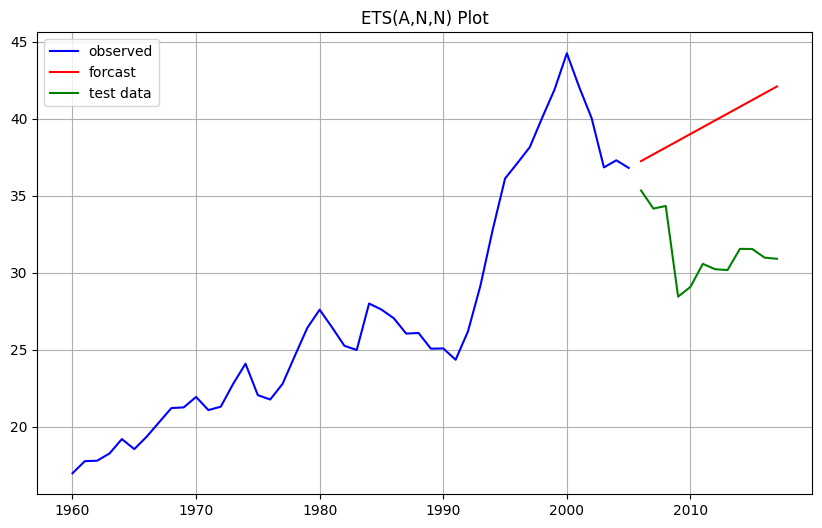
\includegraphics{hw5_files/figure-pdf/cell-17-output-1.png}

\subsubsection{Part C}\label{part-c}

Compute the RMSE values for the training data.

\begin{Shaded}
\begin{Highlighting}[]

\NormalTok{fitted\_values }\OperatorTok{=}\NormalTok{ ets\_model.fittedvalues}
\end{Highlighting}
\end{Shaded}

\begin{Shaded}
\begin{Highlighting}[]
\ImportTok{from}\NormalTok{ sklearn.metrics }\ImportTok{import}\NormalTok{ mean\_squared\_error}
\NormalTok{ann\_rmse }\OperatorTok{=}\NormalTok{ mean\_squared\_error(train\_data, fitted\_values)}

\BuiltInTok{print}\NormalTok{(}\SpecialStringTok{f\textquotesingle{}RMSE: }\SpecialCharTok{\{}\NormalTok{mean\_squared\_error(train\_data, fitted\_values)}\SpecialCharTok{\}}\SpecialStringTok{\textquotesingle{}}\NormalTok{)}
\end{Highlighting}
\end{Shaded}

\begin{verbatim}
RMSE: 2.1710919202650967
\end{verbatim}

\subsubsection{Part D}\label{part-d}

Compare the results to those from an ETS(A,A,N) model. (Remember that
the trended model is using one more parameter than the simpler model.)
Discuss the merits of the two forecasting methods for this data set.

\begin{Shaded}
\begin{Highlighting}[]
\CommentTok{\# for this it is trend =\textquotesingle{}add\textquotesingle{} and damped\_trend = True}

\NormalTok{model }\OperatorTok{=}\NormalTok{ ETSModel(train\_data[}\StringTok{\textquotesingle{}Exports\textquotesingle{}}\NormalTok{], trend }\OperatorTok{=} \StringTok{\textquotesingle{}add\textquotesingle{}}\NormalTok{, damped\_trend}\OperatorTok{=}\VariableTok{True}\NormalTok{, seasonal}\OperatorTok{=}\VariableTok{None}\NormalTok{).fit()}

\NormalTok{aan\_forecast }\OperatorTok{=}\NormalTok{ model.forecast(steps }\OperatorTok{=} \BuiltInTok{len}\NormalTok{(test\_data))}
\end{Highlighting}
\end{Shaded}

\begin{verbatim}
c:\Users\nickc\DataScience\ds_env\Lib\site-packages\statsmodels\tsa\base\tsa_model.py:473: ValueWarning: No frequency information was provided, so inferred frequency AS-JAN will be used.
  self._init_dates(dates, freq)
\end{verbatim}

\begin{Shaded}
\begin{Highlighting}[]
\NormalTok{plt.plot(train\_data.index, train\_data, color }\OperatorTok{=} \StringTok{\textquotesingle{}blue\textquotesingle{}}\NormalTok{, label}\OperatorTok{=}\StringTok{\textquotesingle{}observed\textquotesingle{}}\NormalTok{)}
\NormalTok{plt.plot(aan\_forecast.index, aan\_forecast, color }\OperatorTok{=} \StringTok{\textquotesingle{}red\textquotesingle{}}\NormalTok{, label}\OperatorTok{=}\StringTok{\textquotesingle{}forcast\textquotesingle{}}\NormalTok{)}
\NormalTok{plt.plot(test\_data.index, test\_data, color }\OperatorTok{=} \StringTok{\textquotesingle{}green\textquotesingle{}}\NormalTok{, label}\OperatorTok{=}\StringTok{\textquotesingle{}test data\textquotesingle{}}\NormalTok{)}

\NormalTok{plt.legend(loc }\OperatorTok{=} \StringTok{\textquotesingle{}upper left\textquotesingle{}}\NormalTok{)}
\NormalTok{plt.title(}\StringTok{\textquotesingle{}ETS(A,A,N) Plot\textquotesingle{}}\NormalTok{)}
\NormalTok{plt.grid(}\VariableTok{True}\NormalTok{)}
\NormalTok{plt.show()}
\end{Highlighting}
\end{Shaded}

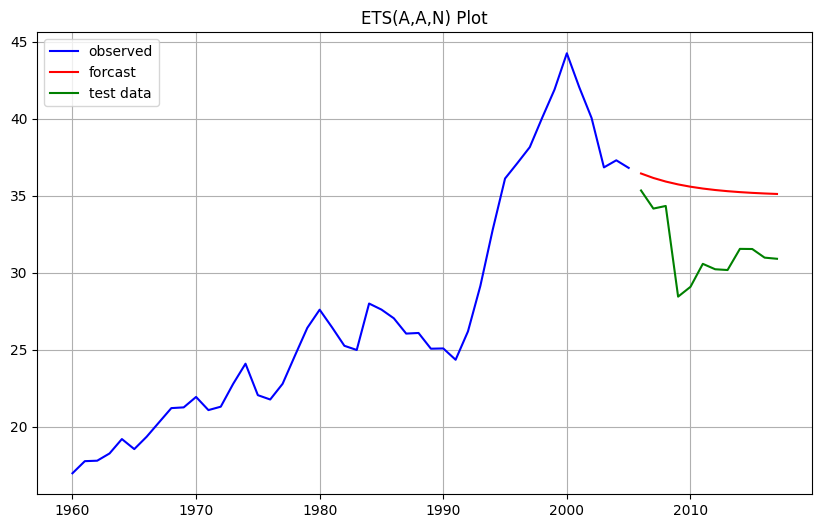
\includegraphics{hw5_files/figure-pdf/cell-21-output-1.png}

\begin{Shaded}
\begin{Highlighting}[]
\NormalTok{fitted\_values }\OperatorTok{=}\NormalTok{ model.fittedvalues}
\NormalTok{aan\_rmse }\OperatorTok{=}\NormalTok{ mean\_squared\_error(train\_data, fitted\_values)}
\BuiltInTok{print}\NormalTok{(}\SpecialStringTok{f\textquotesingle{}RMSE: }\SpecialCharTok{\{}\NormalTok{mean\_squared\_error(train\_data, fitted\_values)}\SpecialCharTok{\}}\SpecialStringTok{\textquotesingle{}}\NormalTok{)}
\end{Highlighting}
\end{Shaded}

\begin{verbatim}
RMSE: 1.9496787243825957
\end{verbatim}

\subsubsection{Part E}\label{part-e}

Compare the forecasts from both methods. Which do you think is best?

Based on the forecasts, we conclude that ETS(A,A,N) provides a better
fit for out timeseries. Not only does its capture the observed downward
trend of the test set, but this is also supported by its lower RMSE
compared to the ETS(A,N,N) model's RMSE. The ETS(A,N,N) model's
assumption of the constant trend leads to an incorrent forecast
trajectory following the training set. highlinhting the importance of
choosing a the correct model.

\subsubsection{Part F}\label{part-f}

Calculate a 95\% prediction interval for the first forecast for each
model, using the RMSE values and assuming normal errors. Compare your
intervals with those produced using R.

\begin{Shaded}
\begin{Highlighting}[]
\NormalTok{ann\_forecast }\OperatorTok{=}\NormalTok{ forecast.iloc[}\DecValTok{0}\NormalTok{]}
\NormalTok{aan\_forecast\_val  }\OperatorTok{=}\NormalTok{ aan\_forecast.iloc[}\DecValTok{0}\NormalTok{]}

\NormalTok{z\_value }\OperatorTok{=} \FloatTok{1.96} \CommentTok{\# for 95 percent }

\NormalTok{prediction\_interval }\OperatorTok{=}\NormalTok{ (ann\_forecast }\OperatorTok{{-}}\NormalTok{ z\_value }\OperatorTok{*}\NormalTok{ ann\_rmse, ann\_forecast }\OperatorTok{+}\NormalTok{ z\_value }\OperatorTok{*}\NormalTok{ ann\_rmse)}
\NormalTok{prediction\_interval\_2 }\OperatorTok{=}\NormalTok{ (aan\_forecast\_val }\OperatorTok{{-}}\NormalTok{ z\_value }\OperatorTok{*}\NormalTok{ aan\_rmse, aan\_forecast\_val }\OperatorTok{+}\NormalTok{ z\_value }\OperatorTok{*}\NormalTok{ aan\_rmse)}
\end{Highlighting}
\end{Shaded}

\begin{Shaded}
\begin{Highlighting}[]

\BuiltInTok{print}\NormalTok{(}\StringTok{\textquotesingle{}Confidence Interval of the first forecast of the ETS(A,N,N) model: \textquotesingle{}}\NormalTok{)}
\BuiltInTok{print}\NormalTok{(prediction\_interval)}
\end{Highlighting}
\end{Shaded}

\begin{verbatim}
Confidence Interval of the first forecast of the ETS(A,N,N) model: 
(32.980483846327374, 41.49116417376655)
\end{verbatim}

\begin{Shaded}
\begin{Highlighting}[]
\BuiltInTok{print}\NormalTok{(}\StringTok{\textquotesingle{}Confidence Interval of the first forecast of the ETS(A,N,N) model: \textquotesingle{}}\NormalTok{)}
\BuiltInTok{print}\NormalTok{(prediction\_interval\_2)}
\end{Highlighting}
\end{Shaded}

\begin{verbatim}
Confidence Interval of the first forecast of the ETS(A,N,N) model: 
(32.61034478739475, 40.25308538697453)
\end{verbatim}

\begin{center}\rule{0.5\linewidth}{0.5pt}\end{center}

\subsection{Exercise 8.6}\label{exercise-8.6}

Forecast the Chinese GDP from the \texttt{global\_economy} data set
using an ETS model. Experiment with the various options in the ETS()
function to see how much the forecasts change with damped trend, or with
a Box-Cox transformation. Try to develop an intuition of what each is
doing to the forecasts.

{[}Hint: use a relatively large value of h when forecasting, so you can
clearly see the differences between the various options when plotting
the forecasts.{]}

\begin{Shaded}
\begin{Highlighting}[]
\NormalTok{china\_gdp }\OperatorTok{=}\NormalTok{ global\_economy.query(}\StringTok{\textquotesingle{}Country == "China"\textquotesingle{}}\NormalTok{)[[}\StringTok{\textquotesingle{}GDP\textquotesingle{}}\NormalTok{]]}
\end{Highlighting}
\end{Shaded}

\begin{Shaded}
\begin{Highlighting}[]
\NormalTok{china\_gdp.plot()}
\NormalTok{plt.grid(}\VariableTok{True}\NormalTok{)}
\NormalTok{plt.show()}
\end{Highlighting}
\end{Shaded}

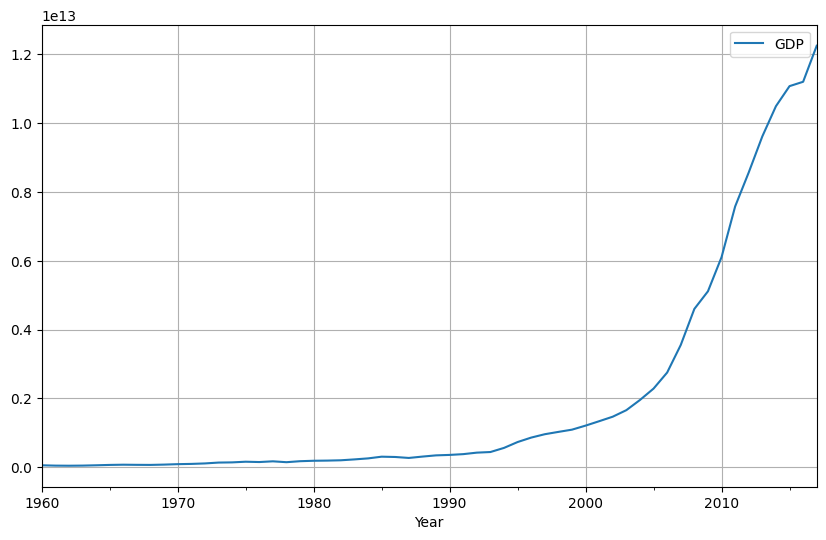
\includegraphics{hw5_files/figure-pdf/cell-28-output-1.png}

\begin{Shaded}
\begin{Highlighting}[]
\NormalTok{train\_data, test\_data }\OperatorTok{=}\NormalTok{ china\_gdp[}\DecValTok{0}\NormalTok{:}\BuiltInTok{int}\NormalTok{(}\BuiltInTok{len}\NormalTok{(china\_gdp)}\OperatorTok{*}\FloatTok{0.8}\NormalTok{) }\OperatorTok{+}\DecValTok{1}\NormalTok{], china\_gdp[}\BuiltInTok{int}\NormalTok{(}\BuiltInTok{len}\NormalTok{(china\_gdp)}\OperatorTok{*}\FloatTok{0.8}\NormalTok{):]}
\end{Highlighting}
\end{Shaded}

\begin{Shaded}
\begin{Highlighting}[]
\CommentTok{\# base model}
\NormalTok{model\_1 }\OperatorTok{=}\NormalTok{ ETSModel(train\_data[}\StringTok{\textquotesingle{}GDP\textquotesingle{}}\NormalTok{], trend}\OperatorTok{=}\StringTok{\textquotesingle{}add\textquotesingle{}}\NormalTok{, seasonal}\OperatorTok{=}\VariableTok{None}\NormalTok{).fit()}

\NormalTok{forecast\_1 }\OperatorTok{=}\NormalTok{ model\_1.forecast(steps}\OperatorTok{=}\BuiltInTok{len}\NormalTok{(test\_data))}
\end{Highlighting}
\end{Shaded}

\begin{verbatim}
c:\Users\nickc\DataScience\ds_env\Lib\site-packages\statsmodels\tsa\base\tsa_model.py:473: ValueWarning: No frequency information was provided, so inferred frequency AS-JAN will be used.
  self._init_dates(dates, freq)
\end{verbatim}

\begin{Shaded}
\begin{Highlighting}[]
\CommentTok{\# with the damped trend }

\NormalTok{model\_2 }\OperatorTok{=}\NormalTok{ ETSModel(train\_data[}\StringTok{\textquotesingle{}GDP\textquotesingle{}}\NormalTok{], trend }\OperatorTok{=} \StringTok{\textquotesingle{}add\textquotesingle{}}\NormalTok{, damped\_trend}\OperatorTok{=}\VariableTok{True}\NormalTok{, seasonal}\OperatorTok{=}\VariableTok{None}\NormalTok{).fit()}

\NormalTok{forecast\_2 }\OperatorTok{=}\NormalTok{ model\_2.forecast(steps }\OperatorTok{=} \BuiltInTok{len}\NormalTok{(test\_data))}
\end{Highlighting}
\end{Shaded}

\begin{verbatim}
c:\Users\nickc\DataScience\ds_env\Lib\site-packages\statsmodels\tsa\base\tsa_model.py:473: ValueWarning: No frequency information was provided, so inferred frequency AS-JAN will be used.
  self._init_dates(dates, freq)
\end{verbatim}

\begin{Shaded}
\begin{Highlighting}[]
\CommentTok{\# box{-}cox transformation}
\ImportTok{from}\NormalTok{ scipy.stats }\ImportTok{import}\NormalTok{ boxcox}
\ImportTok{from}\NormalTok{ scipy.special }\ImportTok{import}\NormalTok{ inv\_boxcox1p}

\NormalTok{gdp\_transformed, lmbda }\OperatorTok{=}\NormalTok{ boxcox(train\_data[}\StringTok{\textquotesingle{}GDP\textquotesingle{}}\NormalTok{]) }\CommentTok{\#| type: ignore}

\NormalTok{train\_data[}\StringTok{\textquotesingle{}gdp\_boxcox\textquotesingle{}}\NormalTok{] }\OperatorTok{=}\NormalTok{ gdp\_transformed}

\NormalTok{model\_3 }\OperatorTok{=}\NormalTok{ ETSModel(train\_data[}\StringTok{\textquotesingle{}gdp\_boxcox\textquotesingle{}}\NormalTok{], trend }\OperatorTok{=} \StringTok{\textquotesingle{}add\textquotesingle{}}\NormalTok{, seasonal }\OperatorTok{=} \VariableTok{None}\NormalTok{).fit()}

\NormalTok{forecast\_3 }\OperatorTok{=}\NormalTok{ model\_3.forecast(steps }\OperatorTok{=} \BuiltInTok{len}\NormalTok{(test\_data))}
\NormalTok{forecast\_3 }\OperatorTok{=}\NormalTok{ inv\_boxcox1p(forecast\_3, lmbda) }\CommentTok{\# undo the tranfromation}
\end{Highlighting}
\end{Shaded}

\begin{verbatim}
C:\Users\nickc\AppData\Local\Temp\ipykernel_28708\3408299051.py:7: SettingWithCopyWarning: 
A value is trying to be set on a copy of a slice from a DataFrame.
Try using .loc[row_indexer,col_indexer] = value instead

See the caveats in the documentation: https://pandas.pydata.org/pandas-docs/stable/user_guide/indexing.html#returning-a-view-versus-a-copy
  train_data['gdp_boxcox'] = gdp_transformed
c:\Users\nickc\DataScience\ds_env\Lib\site-packages\statsmodels\tsa\base\tsa_model.py:473: ValueWarning: No frequency information was provided, so inferred frequency AS-JAN will be used.
  self._init_dates(dates, freq)
\end{verbatim}

\begin{Shaded}
\begin{Highlighting}[]
\CommentTok{\# log transform with damped}

\NormalTok{train\_data.loc[:, }\StringTok{\textquotesingle{}log\_gdp\textquotesingle{}}\NormalTok{] }\OperatorTok{=}\NormalTok{ np.log(train\_data[}\StringTok{\textquotesingle{}GDP\textquotesingle{}}\NormalTok{]).copy() }

\NormalTok{model\_4 }\OperatorTok{=}\NormalTok{ ETSModel(train\_data[}\StringTok{\textquotesingle{}log\_gdp\textquotesingle{}}\NormalTok{], trend }\OperatorTok{=} \StringTok{\textquotesingle{}add\textquotesingle{}}\NormalTok{, damped\_trend}\OperatorTok{=} \VariableTok{True}\NormalTok{, seasonal }\OperatorTok{=} \VariableTok{None}\NormalTok{).fit()}

\NormalTok{forecast\_4 }\OperatorTok{=}\NormalTok{ model\_4.forecast(steps}\OperatorTok{=} \BuiltInTok{len}\NormalTok{(test\_data))}
\NormalTok{forecast\_4 }\OperatorTok{=}\NormalTok{ np.exp(forecast\_4)}
\end{Highlighting}
\end{Shaded}

\begin{verbatim}
C:\Users\nickc\AppData\Local\Temp\ipykernel_28708\3159823729.py:3: SettingWithCopyWarning: 
A value is trying to be set on a copy of a slice from a DataFrame.
Try using .loc[row_indexer,col_indexer] = value instead

See the caveats in the documentation: https://pandas.pydata.org/pandas-docs/stable/user_guide/indexing.html#returning-a-view-versus-a-copy
  train_data.loc[:, 'log_gdp'] = np.log(train_data['GDP']).copy()
c:\Users\nickc\DataScience\ds_env\Lib\site-packages\statsmodels\tsa\base\tsa_model.py:473: ValueWarning: No frequency information was provided, so inferred frequency AS-JAN will be used.
  self._init_dates(dates, freq)
\end{verbatim}

\begin{Shaded}
\begin{Highlighting}[]
\NormalTok{train\_data[}\StringTok{\textquotesingle{}GDP\textquotesingle{}}\NormalTok{].plot(label}\OperatorTok{=}\StringTok{\textquotesingle{}Original\textquotesingle{}}\NormalTok{, color }\OperatorTok{=} \StringTok{\textquotesingle{}grey\textquotesingle{}}\NormalTok{)}
\NormalTok{forecast\_1.plot(label}\OperatorTok{=}\StringTok{\textquotesingle{}Base ETS\textquotesingle{}}\NormalTok{, color }\OperatorTok{=} \StringTok{\textquotesingle{}purple\textquotesingle{}}\NormalTok{)}
\NormalTok{forecast\_2.plot(label}\OperatorTok{=}\StringTok{\textquotesingle{}ETS with Damped Trend\textquotesingle{}}\NormalTok{, color }\OperatorTok{=}\StringTok{\textquotesingle{}blue\textquotesingle{}}\NormalTok{)}
\NormalTok{forecast\_3.plot(label}\OperatorTok{=}\StringTok{\textquotesingle{}ETS with Box{-}Cox\textquotesingle{}}\NormalTok{, color }\OperatorTok{=} \StringTok{\textquotesingle{}green\textquotesingle{}}\NormalTok{)}
\NormalTok{forecast\_4.plot(label}\OperatorTok{=} \StringTok{\textquotesingle{}ETS with Log and Damped Trend\textquotesingle{}}\NormalTok{, color }\OperatorTok{=} \StringTok{\textquotesingle{}pink\textquotesingle{}}\NormalTok{)}
\NormalTok{test\_data[}\StringTok{\textquotesingle{}GDP\textquotesingle{}}\NormalTok{].plot(label }\OperatorTok{=} \StringTok{\textquotesingle{}Observed Test Data\textquotesingle{}}\NormalTok{, color }\OperatorTok{=} \StringTok{\textquotesingle{}red\textquotesingle{}}\NormalTok{)}
\NormalTok{plt.legend()}
\NormalTok{plt.title(}\StringTok{\textquotesingle{}Chinese GDP Forecasts\textquotesingle{}}\NormalTok{)}
\NormalTok{plt.grid(}\VariableTok{True}\NormalTok{)}
\NormalTok{plt.show()}
\end{Highlighting}
\end{Shaded}

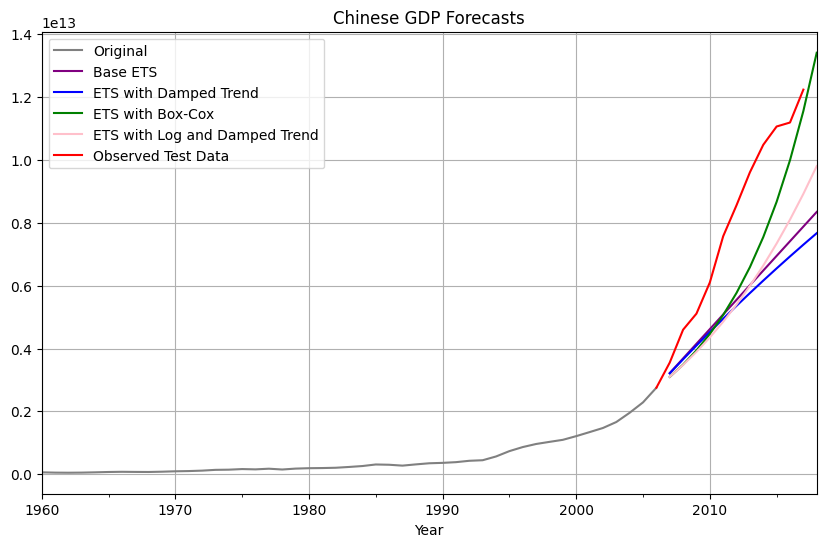
\includegraphics{hw5_files/figure-pdf/cell-34-output-1.png}

The base model with simple exponential smoothing captures the general
upward trend of China's GDP. However, as the base model it might not
capture the growth rate of the data since the appears to be linear. The
dampening factor smooths out the trend. This introduces the intuition
that the explosive growth rate observed in the past might slow down in
the future. The forecast reflects a less steep trajectory. The Box-Cox
transformation often helps when the pattern of increase in a time series
changes over time. In this case, since it fits the test data closely,
the intuition is that Chinese GDP might have a pattern of increasingly
rapid growth that the standard ETS model wasn't fully capturing. The log
transformation tends to scale down large values. In combination with
dampening, this model intuitively suggests a very conservative forecast
but knows that growth exists, but will progress much slower than any of
the other models project.

\begin{center}\rule{0.5\linewidth}{0.5pt}\end{center}

\subsection{Exercise 8.7}\label{exercise-8.7}

Find an ETS model for the Gas data from \texttt{aus\_production} and
forecast the next few years. Why is multiplicative seasonality necessary
here? Experiment with making the trend damped. Does it improve the
forecasts?

\begin{Shaded}
\begin{Highlighting}[]
\NormalTok{aus\_gas }\OperatorTok{=}\NormalTok{ aus\_production[[}\StringTok{\textquotesingle{}Gas\textquotesingle{}}\NormalTok{]]}
\end{Highlighting}
\end{Shaded}

\begin{Shaded}
\begin{Highlighting}[]
\NormalTok{aus\_gas.plot()}
\NormalTok{plt.grid(}\VariableTok{True}\NormalTok{)}
\NormalTok{plt.show()}
\end{Highlighting}
\end{Shaded}

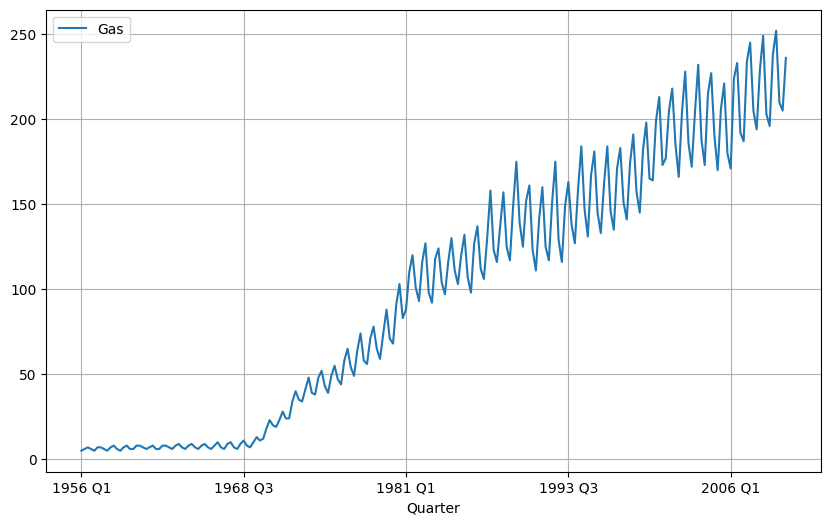
\includegraphics{hw5_files/figure-pdf/cell-37-output-1.png}

The Gas production data displays an increasing variance pattern over
time. This means that the magnitude of the fluctuations and the impact
of the trend component likely scale with the underlying production
level. Therefore, a multiplicative ETS model is expected to better
capture this behavior and generate more reliable forecasts.

\begin{Shaded}
\begin{Highlighting}[]
\NormalTok{train\_data, test\_data }\OperatorTok{=}\NormalTok{ aus\_gas[}\DecValTok{0}\NormalTok{:}\BuiltInTok{int}\NormalTok{(}\BuiltInTok{len}\NormalTok{(aus\_gas)}\OperatorTok{*}\FloatTok{0.8}\NormalTok{) }\OperatorTok{+}\DecValTok{1}\NormalTok{], aus\_gas[}\BuiltInTok{int}\NormalTok{(}\BuiltInTok{len}\NormalTok{(aus\_gas)}\OperatorTok{*}\FloatTok{0.8}\NormalTok{):]}
\end{Highlighting}
\end{Shaded}

\begin{Shaded}
\begin{Highlighting}[]
\CommentTok{\# base model}
\NormalTok{model }\OperatorTok{=}\NormalTok{ ETSModel(train\_data[}\StringTok{\textquotesingle{}Gas\textquotesingle{}}\NormalTok{], trend }\OperatorTok{=} \StringTok{\textquotesingle{}add\textquotesingle{}}\NormalTok{).fit()}

\NormalTok{forecast\_base }\OperatorTok{=}\NormalTok{ model.forecast(steps }\OperatorTok{=} \BuiltInTok{len}\NormalTok{(test\_data))}
\end{Highlighting}
\end{Shaded}

\begin{verbatim}
c:\Users\nickc\DataScience\ds_env\Lib\site-packages\statsmodels\tsa\base\tsa_model.py:559: UserWarning: Could not infer format, so each element will be parsed individually, falling back to `dateutil`. To ensure parsing is consistent and as-expected, please specify a format.
  _index = to_datetime(index)
c:\Users\nickc\DataScience\ds_env\Lib\site-packages\statsmodels\tsa\base\tsa_model.py:473: ValueWarning: An unsupported index was provided and will be ignored when e.g. forecasting.
  self._init_dates(dates, freq)
c:\Users\nickc\DataScience\ds_env\Lib\site-packages\statsmodels\tsa\base\tsa_model.py:836: ValueWarning: No supported index is available. Prediction results will be given with an integer index beginning at `start`.
  return get_prediction_index(
c:\Users\nickc\DataScience\ds_env\Lib\site-packages\statsmodels\tsa\base\tsa_model.py:836: FutureWarning: No supported index is available. In the next version, calling this method in a model without a supported index will result in an exception.
  return get_prediction_index(
\end{verbatim}

\begin{Shaded}
\begin{Highlighting}[]
\CommentTok{\#  change seasonal to multiplicative}
\NormalTok{model\_mul }\OperatorTok{=}\NormalTok{ ETSModel(train\_data[}\StringTok{\textquotesingle{}Gas\textquotesingle{}}\NormalTok{], trend }\OperatorTok{=} \StringTok{\textquotesingle{}add\textquotesingle{}}\NormalTok{, seasonal }\OperatorTok{=} \StringTok{\textquotesingle{}mul\textquotesingle{}}\NormalTok{, seasonal\_periods }\OperatorTok{=} \DecValTok{4}\NormalTok{).fit()}

\NormalTok{forecast\_mul }\OperatorTok{=}\NormalTok{ model\_mul.forecast(steps }\OperatorTok{=} \BuiltInTok{len}\NormalTok{(test\_data))}
\end{Highlighting}
\end{Shaded}

\begin{verbatim}
c:\Users\nickc\DataScience\ds_env\Lib\site-packages\statsmodels\tsa\base\tsa_model.py:559: UserWarning: Could not infer format, so each element will be parsed individually, falling back to `dateutil`. To ensure parsing is consistent and as-expected, please specify a format.
  _index = to_datetime(index)
c:\Users\nickc\DataScience\ds_env\Lib\site-packages\statsmodels\tsa\base\tsa_model.py:473: ValueWarning: An unsupported index was provided and will be ignored when e.g. forecasting.
  self._init_dates(dates, freq)
c:\Users\nickc\DataScience\ds_env\Lib\site-packages\statsmodels\tsa\base\tsa_model.py:836: ValueWarning: No supported index is available. Prediction results will be given with an integer index beginning at `start`.
  return get_prediction_index(
c:\Users\nickc\DataScience\ds_env\Lib\site-packages\statsmodels\tsa\base\tsa_model.py:836: FutureWarning: No supported index is available. In the next version, calling this method in a model without a supported index will result in an exception.
  return get_prediction_index(
\end{verbatim}

\begin{Shaded}
\begin{Highlighting}[]
\NormalTok{model\_damped }\OperatorTok{=}\NormalTok{ ETSModel(train\_data[}\StringTok{\textquotesingle{}Gas\textquotesingle{}}\NormalTok{], trend }\OperatorTok{=} \StringTok{\textquotesingle{}add\textquotesingle{}}\NormalTok{, damped\_trend}\OperatorTok{=}\VariableTok{True}\NormalTok{, seasonal }\OperatorTok{=} \StringTok{\textquotesingle{}mul\textquotesingle{}}\NormalTok{, seasonal\_periods }\OperatorTok{=} \DecValTok{4}\NormalTok{).fit()}

\NormalTok{forecast\_damped }\OperatorTok{=}\NormalTok{ model\_damped.forecast(steps }\OperatorTok{=} \BuiltInTok{len}\NormalTok{(test\_data))}
\end{Highlighting}
\end{Shaded}

\begin{verbatim}
c:\Users\nickc\DataScience\ds_env\Lib\site-packages\statsmodels\tsa\base\tsa_model.py:559: UserWarning: Could not infer format, so each element will be parsed individually, falling back to `dateutil`. To ensure parsing is consistent and as-expected, please specify a format.
  _index = to_datetime(index)
c:\Users\nickc\DataScience\ds_env\Lib\site-packages\statsmodels\tsa\base\tsa_model.py:473: ValueWarning: An unsupported index was provided and will be ignored when e.g. forecasting.
  self._init_dates(dates, freq)
c:\Users\nickc\DataScience\ds_env\Lib\site-packages\statsmodels\tsa\base\tsa_model.py:836: ValueWarning: No supported index is available. Prediction results will be given with an integer index beginning at `start`.
  return get_prediction_index(
c:\Users\nickc\DataScience\ds_env\Lib\site-packages\statsmodels\tsa\base\tsa_model.py:836: FutureWarning: No supported index is available. In the next version, calling this method in a model without a supported index will result in an exception.
  return get_prediction_index(
\end{verbatim}

\begin{Shaded}
\begin{Highlighting}[]
\NormalTok{aus\_gas.plot(label}\OperatorTok{=}\StringTok{\textquotesingle{}Observed Data\textquotesingle{}}\NormalTok{, color }\OperatorTok{=} \StringTok{\textquotesingle{}grey\textquotesingle{}}\NormalTok{)}
\NormalTok{forecast\_base.plot(label }\OperatorTok{=} \StringTok{\textquotesingle{}Base Forecast\textquotesingle{}}\NormalTok{, color }\OperatorTok{=} \StringTok{\textquotesingle{}red\textquotesingle{}}\NormalTok{)}
\NormalTok{forecast\_mul.plot(label }\OperatorTok{=} \StringTok{\textquotesingle{}Multiplicative Forecast\textquotesingle{}}\NormalTok{, color }\OperatorTok{=} \StringTok{\textquotesingle{}green\textquotesingle{}}\NormalTok{)}
\NormalTok{forecast\_damped.plot(label }\OperatorTok{=} \StringTok{\textquotesingle{}Damped Forecast\textquotesingle{}}\NormalTok{, color }\OperatorTok{=} \StringTok{\textquotesingle{}orange\textquotesingle{}}\NormalTok{)}

\NormalTok{plt.legend()}
\NormalTok{plt.grid(}\VariableTok{True}\NormalTok{)}
\NormalTok{plt.show()}
\end{Highlighting}
\end{Shaded}

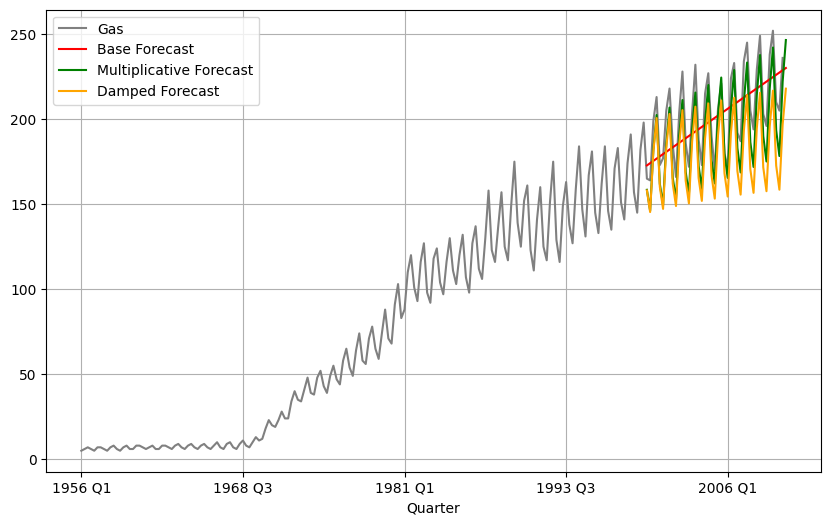
\includegraphics{hw5_files/figure-pdf/cell-42-output-1.png}

The damped trend into the ETS model results in a more conservative trend
forecast, suggesting a potential slowdown in the growth rate compared to
the basic ETS model. While the multiplicative seasonal ETS model appears
to align more closely with the observed data patterns than the damped
forecast.Thus, indicates that the variance in the time series might
increase along with the overall level, making the multiplicative
seasonality model a better fit.

\begin{center}\rule{0.5\linewidth}{0.5pt}\end{center}

\subsection{Exercise 8.8}\label{exercise-8.8}

Recall your retail time series data (from Exercise 7 in Section 2.10).

\begin{verbatim}
C:\Users\nickc\AppData\Local\Temp\ipykernel_28708\3632377730.py:2: UserWarning: Could not infer format, so each element will be parsed individually, falling back to `dateutil`. To ensure parsing is consistent and as-expected, please specify a format.
  aus_retail = pd.read_csv('c:/Users/nickc/DataScience/NickAMC.github.io/DATA_624_S24/rdata/aus_retail.csv', parse_dates=['Month'], index_col='Month')
\end{verbatim}

\begin{Shaded}
\begin{Highlighting}[]
\NormalTok{aus\_retail.State.unique()}
\end{Highlighting}
\end{Shaded}

\begin{verbatim}
array(['Australian Capital Territory', 'New South Wales',
       'Northern Territory', 'Queensland', 'South Australia', 'Tasmania',
       'Victoria', 'Western Australia'], dtype=object)
\end{verbatim}

\begin{Shaded}
\begin{Highlighting}[]
\NormalTok{clothing\_retail }\OperatorTok{=}\NormalTok{ aus\_retail.query(}\StringTok{\textquotesingle{}Industry == "Clothing retailing" \& State == "Australian Capital Territory"\textquotesingle{}}\NormalTok{)[[}\StringTok{\textquotesingle{}Turnover\textquotesingle{}}\NormalTok{]]}
\end{Highlighting}
\end{Shaded}

\subsubsection{Part A}\label{part-a-2}

Why is multiplicative seasonality necessary for this series?

\begin{Shaded}
\begin{Highlighting}[]
\NormalTok{clothing\_retail.plot()}
\NormalTok{plt.show()}
\end{Highlighting}
\end{Shaded}

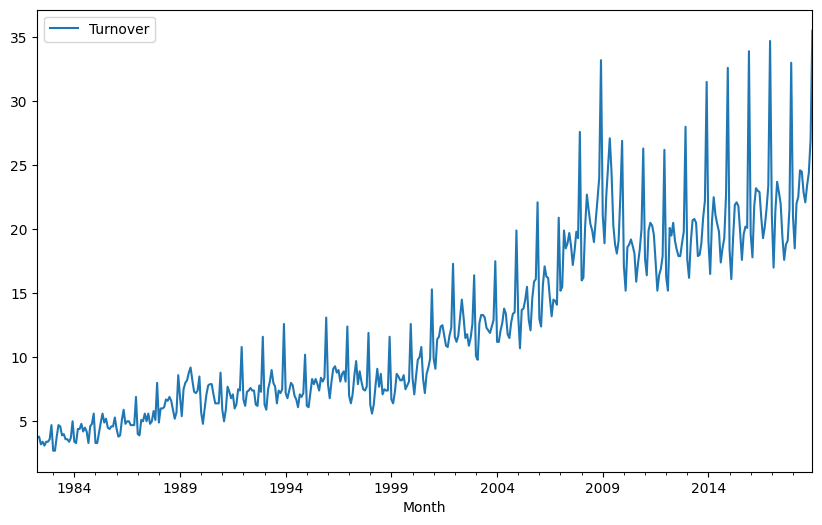
\includegraphics{hw5_files/figure-pdf/cell-46-output-1.png}

\begin{Shaded}
\begin{Highlighting}[]
\NormalTok{train, test}\OperatorTok{=}\NormalTok{ clothing\_retail[}\DecValTok{0}\NormalTok{:}\BuiltInTok{int}\NormalTok{(}\BuiltInTok{len}\NormalTok{(clothing\_retail)}\OperatorTok{*}\FloatTok{0.8}\NormalTok{) }\OperatorTok{+}\DecValTok{1}\NormalTok{], clothing\_retail[}\BuiltInTok{int}\NormalTok{(}\BuiltInTok{len}\NormalTok{(clothing\_retail)}\OperatorTok{*}\FloatTok{0.8}\NormalTok{):]}
\end{Highlighting}
\end{Shaded}

\subsubsection{Part B}\label{part-b-2}

Apply Holt-Winters' multiplicative method to the data. Experiment with
making the trend damped.

\begin{Shaded}
\begin{Highlighting}[]
\NormalTok{model}\OperatorTok{=}\NormalTok{ ETSModel(train[}\StringTok{\textquotesingle{}Turnover\textquotesingle{}}\NormalTok{], trend}\OperatorTok{=}\StringTok{\textquotesingle{}add\textquotesingle{}}\NormalTok{, seasonal}\OperatorTok{=}\StringTok{\textquotesingle{}mul\textquotesingle{}}\NormalTok{, damped\_trend}\OperatorTok{=}\VariableTok{False}\NormalTok{).fit()}

\NormalTok{forecast}\OperatorTok{=}\NormalTok{ model.forecast(steps }\OperatorTok{=} \BuiltInTok{len}\NormalTok{(test))}
\end{Highlighting}
\end{Shaded}

\begin{verbatim}
c:\Users\nickc\DataScience\ds_env\Lib\site-packages\statsmodels\tsa\base\tsa_model.py:473: ValueWarning: No frequency information was provided, so inferred frequency MS will be used.
  self._init_dates(dates, freq)
\end{verbatim}

\begin{Shaded}
\begin{Highlighting}[]
\NormalTok{model\_damp }\OperatorTok{=}\NormalTok{ ETSModel(train[}\StringTok{\textquotesingle{}Turnover\textquotesingle{}}\NormalTok{], trend}\OperatorTok{=}\StringTok{\textquotesingle{}add\textquotesingle{}}\NormalTok{, seasonal}\OperatorTok{=}\StringTok{\textquotesingle{}mul\textquotesingle{}}\NormalTok{, damped\_trend}\OperatorTok{=}\VariableTok{True}\NormalTok{).fit()}

\NormalTok{forecast\_damp }\OperatorTok{=}\NormalTok{ model\_damp.forecast(steps }\OperatorTok{=} \BuiltInTok{len}\NormalTok{(test))}
\end{Highlighting}
\end{Shaded}

\begin{verbatim}
c:\Users\nickc\DataScience\ds_env\Lib\site-packages\statsmodels\tsa\base\tsa_model.py:473: ValueWarning: No frequency information was provided, so inferred frequency MS will be used.
  self._init_dates(dates, freq)
\end{verbatim}

\begin{Shaded}
\begin{Highlighting}[]
\NormalTok{clothing\_retail.plot(label }\OperatorTok{=} \StringTok{\textquotesingle{}Observed\textquotesingle{}}\NormalTok{)}
\NormalTok{forecast.plot(label }\OperatorTok{=} \StringTok{\textquotesingle{}Forecast\textquotesingle{}}\NormalTok{, color }\OperatorTok{=} \StringTok{\textquotesingle{}green\textquotesingle{}}\NormalTok{)}
\NormalTok{forecast\_damp.plot(label }\OperatorTok{=} \StringTok{\textquotesingle{}Damped Forecast\textquotesingle{}}\NormalTok{, color }\OperatorTok{=} \StringTok{\textquotesingle{}red\textquotesingle{}}\NormalTok{)}

\NormalTok{plt.legend()}
\NormalTok{plt.grid(}\VariableTok{True}\NormalTok{)}
\NormalTok{plt.show()}
\end{Highlighting}
\end{Shaded}

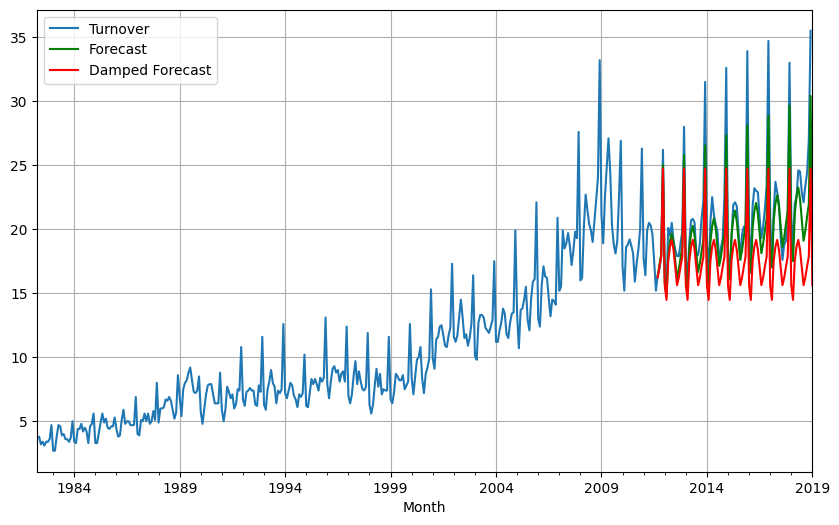
\includegraphics{hw5_files/figure-pdf/cell-50-output-1.png}

\subsubsection{Part C}\label{part-c-1}

Compare the RMSE of the one-step forecasts from the two methods. Which
do you prefer?

\begin{Shaded}
\begin{Highlighting}[]
\ImportTok{from}\NormalTok{ sklearn.metrics }\ImportTok{import}\NormalTok{ mean\_squared\_error}


\NormalTok{rmse }\OperatorTok{=}\NormalTok{ np.sqrt(mean\_squared\_error(test[}\StringTok{\textquotesingle{}Turnover\textquotesingle{}}\NormalTok{], forecast))}
\NormalTok{rmse\_damp }\OperatorTok{=}\NormalTok{ np.sqrt(mean\_squared\_error(test[}\StringTok{\textquotesingle{}Turnover\textquotesingle{}}\NormalTok{], forecast\_damp))}

\BuiltInTok{print}\NormalTok{(}\StringTok{"RMSE (Multiplicative ETS):"}\NormalTok{, rmse)}
\BuiltInTok{print}\NormalTok{(}\StringTok{"RMSE (Damped Multiplicative ETS):"}\NormalTok{, rmse\_damp)}
\end{Highlighting}
\end{Shaded}

\begin{verbatim}
RMSE (Multiplicative ETS): 5.032452417615934
RMSE (Damped Multiplicative ETS): 6.015841153098568
\end{verbatim}

\subsubsection{Part D}\label{part-d-1}

Check that the residuals from the best method look like white noise.

\begin{Shaded}
\begin{Highlighting}[]
\NormalTok{residuals }\OperatorTok{=}\NormalTok{ model.resid}
\NormalTok{residuals.plot()}
\NormalTok{plt.title(}\StringTok{\textquotesingle{}Residuals Time Plot\textquotesingle{}}\NormalTok{)}
\NormalTok{plt.show()}
\end{Highlighting}
\end{Shaded}

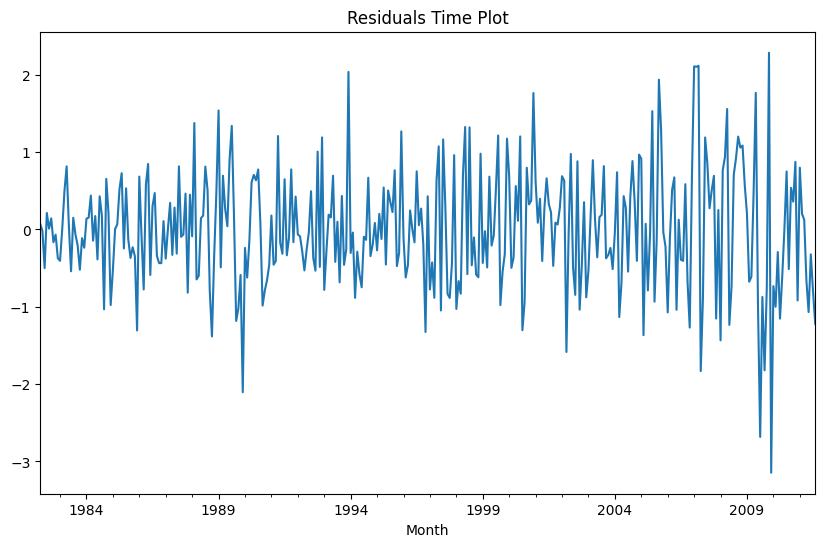
\includegraphics{hw5_files/figure-pdf/cell-52-output-1.png}

\begin{Shaded}
\begin{Highlighting}[]
\NormalTok{residuals.hist()}
\NormalTok{plt.show}
\end{Highlighting}
\end{Shaded}

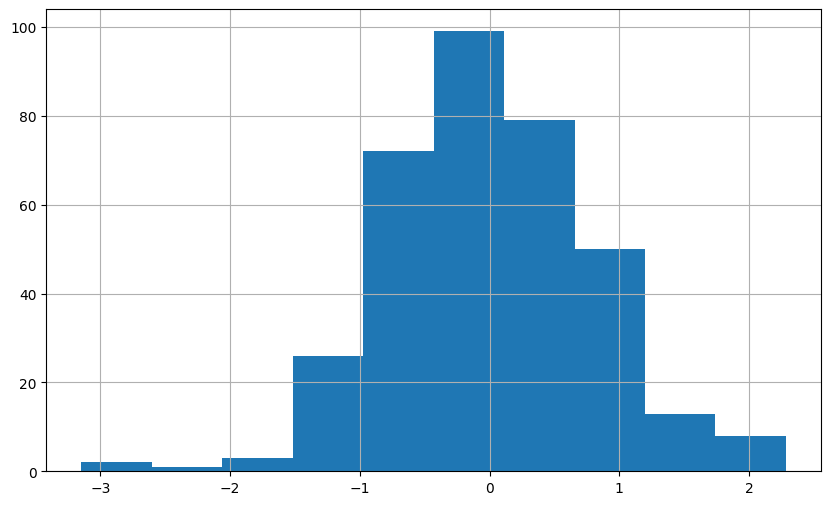
\includegraphics{hw5_files/figure-pdf/cell-53-output-1.png}

Residuals exhibits no clear patterns and appears to be randomly
scatterred around zero.

\begin{Shaded}
\begin{Highlighting}[]
\BuiltInTok{print}\NormalTok{(model.summary())}
\end{Highlighting}
\end{Shaded}

\begin{verbatim}
                                 ETS Results                                  
==============================================================================
Dep. Variable:               Turnover   No. Observations:                  353
Model:                       ETS(AAM)   Log Likelihood                -406.420
Date:                Sun, 03 Mar 2024   AIC                            848.840
Time:                        18:57:51   BIC                            918.437
Sample:                    04-01-1982   HQIC                           876.533
                         - 08-01-2011   Scale                            0.586
Covariance Type:               approx                                         
=======================================================================================
                          coef    std err          z      P>|z|      [0.025      0.975]
---------------------------------------------------------------------------------------
smoothing_level         0.6078      0.069      8.747      0.000       0.472       0.744
smoothing_trend      6.078e-05        nan        nan        nan         nan         nan
smoothing_seasonal   3.922e-05      0.085      0.000      1.000      -0.166       0.166
initial_level           3.5788    154.259      0.023      0.981    -298.763     305.921
initial_trend           0.0488      2.105      0.023      0.981      -4.078       4.175
initial_seasonal.0      0.9403     40.529      0.023      0.981     -78.496      80.376
initial_seasonal.1      0.7779     33.530      0.023      0.981     -64.940      66.495
initial_seasonal.2      0.8369     36.073      0.023      0.981     -69.866      71.539
initial_seasonal.3      1.3232     57.037      0.023      0.981    -110.468     113.114
initial_seasonal.4      0.9580     41.294      0.023      0.981     -79.976      81.892
initial_seasonal.5      0.9168     39.517      0.023      0.981     -76.536      78.370
initial_seasonal.6      0.8706     37.526      0.023      0.981     -72.679      74.420
initial_seasonal.7      0.8383     36.134      0.023      0.981     -69.983      71.660
initial_seasonal.8      0.9117     39.296      0.023      0.981     -76.108      77.931
initial_seasonal.9      0.9851     42.463      0.023      0.981     -82.242      84.212
initial_seasonal.10     1.0269     44.265      0.023      0.981     -85.730      87.784
initial_seasonal.11     1.0000     43.103      0.023      0.981     -83.481      85.481
===================================================================================
Ljung-Box (Q):                       21.06   Jarque-Bera (JB):                13.38
Prob(Q):                              0.64   Prob(JB):                         0.00
Heteroskedasticity (H):               2.67   Skew:                            -0.00
Prob(H) (two-sided):                  0.00   Kurtosis:                         3.95
===================================================================================

Warnings:
[1] Covariance matrix calculated using numerical (complex-step) differentiation.
\end{verbatim}

The Ljung-Box indicates that the residuals are uncorrelated and
Jarque-Bera test rejects the null where the residuals are normality
distributed.

\subsubsection{Part E}\label{part-e-1}

Now find the test set RMSE, while training the model to the end of 2010.
Can you beat the seasonal naïve approach from Exercise 7 in Section
5.11?

\begin{Shaded}
\begin{Highlighting}[]
\NormalTok{train\_2010 }\OperatorTok{=}\NormalTok{ clothing\_retail.loc[:}\StringTok{\textquotesingle{}2010\textquotesingle{}}\NormalTok{]  }
\NormalTok{model\_2010 }\OperatorTok{=}\NormalTok{ ETSModel(train\_2010[}\StringTok{\textquotesingle{}Turnover\textquotesingle{}}\NormalTok{], trend}\OperatorTok{=}\StringTok{\textquotesingle{}add\textquotesingle{}}\NormalTok{, seasonal}\OperatorTok{=}\StringTok{\textquotesingle{}mul\textquotesingle{}}\NormalTok{, damped\_trend}\OperatorTok{=}\VariableTok{True}\NormalTok{).fit() }

\NormalTok{forecast\_2010 }\OperatorTok{=}\NormalTok{ model\_2010.forecast(steps}\OperatorTok{=}\BuiltInTok{len}\NormalTok{(test)) }
\end{Highlighting}
\end{Shaded}

\begin{verbatim}
c:\Users\nickc\DataScience\ds_env\Lib\site-packages\statsmodels\tsa\base\tsa_model.py:473: ValueWarning: No frequency information was provided, so inferred frequency MS will be used.
  self._init_dates(dates, freq)
\end{verbatim}

\begin{Shaded}
\begin{Highlighting}[]
\NormalTok{test\_rmse }\OperatorTok{=}\NormalTok{ np.sqrt(mean\_squared\_error(test[}\StringTok{\textquotesingle{}Turnover\textquotesingle{}}\NormalTok{], forecast\_2010))}
\BuiltInTok{print}\NormalTok{(}\StringTok{"Test Set RMSE (ETS Model):"}\NormalTok{, test\_rmse)}
\end{Highlighting}
\end{Shaded}

\begin{verbatim}
Test Set RMSE (ETS Model): 5.003789852798558
\end{verbatim}

\begin{center}\rule{0.5\linewidth}{0.5pt}\end{center}

\subsection{Exercise 8.9}\label{exercise-8.9}

For the same retail data, try an STL decomposition applied to the
Box-Cox transformed series, followed by ETS on the seasonally adjusted
data. How does that compare with your best previous forecasts on the
test set?

\begin{Shaded}
\begin{Highlighting}[]
\NormalTok{turnover\_boxcox, lmbda }\OperatorTok{=}\NormalTok{ boxcox(train[}\StringTok{\textquotesingle{}Turnover\textquotesingle{}}\NormalTok{])}

\NormalTok{train[}\StringTok{\textquotesingle{}Turnover\_boxcox\textquotesingle{}}\NormalTok{] }\OperatorTok{=}\NormalTok{ turnover\_boxcox}
\end{Highlighting}
\end{Shaded}

\begin{verbatim}
C:\Users\nickc\AppData\Local\Temp\ipykernel_28708\381446324.py:3: SettingWithCopyWarning: 
A value is trying to be set on a copy of a slice from a DataFrame.
Try using .loc[row_indexer,col_indexer] = value instead

See the caveats in the documentation: https://pandas.pydata.org/pandas-docs/stable/user_guide/indexing.html#returning-a-view-versus-a-copy
  train['Turnover_boxcox'] = turnover_boxcox
\end{verbatim}

\begin{Shaded}
\begin{Highlighting}[]
\NormalTok{stl }\OperatorTok{=}\NormalTok{ seasonal\_decompose(train[}\StringTok{\textquotesingle{}Turnover\_boxcox\textquotesingle{}}\NormalTok{], model}\OperatorTok{=}\StringTok{\textquotesingle{}mupltiplicative\textquotesingle{}}\NormalTok{, period}\OperatorTok{=}\DecValTok{12}\NormalTok{) }
\end{Highlighting}
\end{Shaded}

\begin{Shaded}
\begin{Highlighting}[]
\NormalTok{stl.resid.isna().}\BuiltInTok{sum}\NormalTok{()}
\end{Highlighting}
\end{Shaded}

\begin{verbatim}
12
\end{verbatim}

\begin{Shaded}
\begin{Highlighting}[]
\NormalTok{stl.plot()}
\NormalTok{plt.show()}
\end{Highlighting}
\end{Shaded}

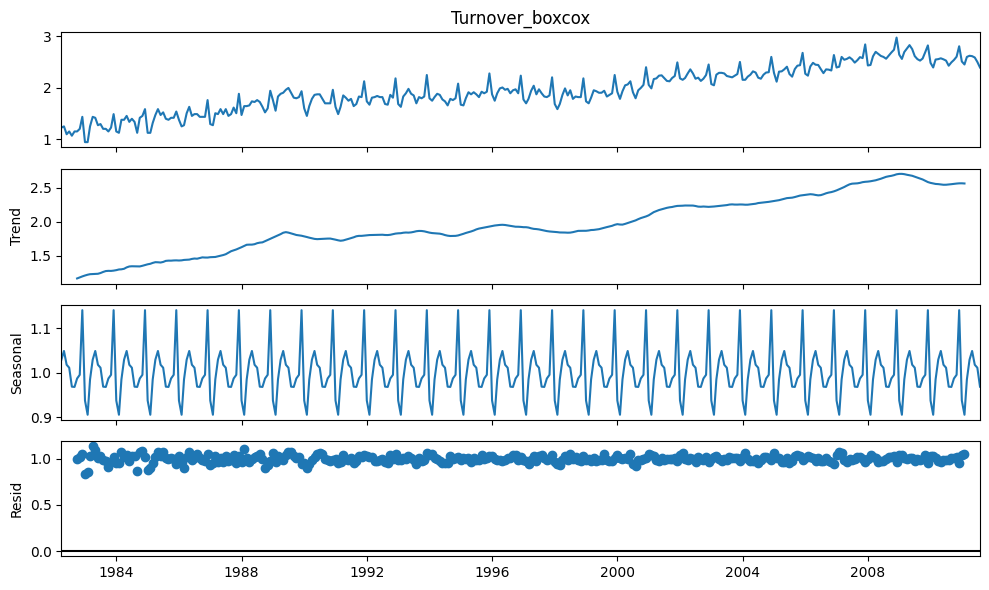
\includegraphics{hw5_files/figure-pdf/cell-60-output-1.png}

\begin{Shaded}
\begin{Highlighting}[]
\NormalTok{test\_decomposed }\OperatorTok{=}\NormalTok{ seasonal\_decompose(train[}\StringTok{\textquotesingle{}Turnover\_boxcox\textquotesingle{}}\NormalTok{], model}\OperatorTok{=}\StringTok{\textquotesingle{}additive\textquotesingle{}}\NormalTok{, period}\OperatorTok{=}\DecValTok{12}\NormalTok{)}
\NormalTok{test\_resid }\OperatorTok{=}\NormalTok{ test\_decomposed.resid.dropna()}
\end{Highlighting}
\end{Shaded}

\begin{Shaded}
\begin{Highlighting}[]
\NormalTok{model\_ets }\OperatorTok{=}\NormalTok{ ExponentialSmoothing(stl.resid.dropna() }\OperatorTok{+} \FloatTok{0.001}\NormalTok{, trend}\OperatorTok{=}\StringTok{\textquotesingle{}add\textquotesingle{}}\NormalTok{, seasonal}\OperatorTok{=}\StringTok{\textquotesingle{}mul\textquotesingle{}}\NormalTok{, seasonal\_periods}\OperatorTok{=}\DecValTok{12}\NormalTok{).fit()}

\NormalTok{forecast}\OperatorTok{=}\NormalTok{ model\_ets.forecast(steps}\OperatorTok{=}\BuiltInTok{len}\NormalTok{(test\_resid))}

\NormalTok{forecast }\OperatorTok{=}\NormalTok{ inv\_boxcox1p(forecast, lmbda)}
\end{Highlighting}
\end{Shaded}

\begin{verbatim}
c:\Users\nickc\DataScience\ds_env\Lib\site-packages\statsmodels\tsa\base\tsa_model.py:473: ValueWarning: No frequency information was provided, so inferred frequency MS will be used.
  self._init_dates(dates, freq)
\end{verbatim}

\begin{Shaded}
\begin{Highlighting}[]
\NormalTok{test\_rmse }\OperatorTok{=}\NormalTok{ np.sqrt(mean\_squared\_error(test\_resid, forecast))}
\BuiltInTok{print}\NormalTok{(}\StringTok{"Test Set RMSE (ETS Model):"}\NormalTok{, test\_rmse)}
\end{Highlighting}
\end{Shaded}

\begin{verbatim}
Test Set RMSE (ETS Model): 1.8695669650523843
\end{verbatim}



\end{document}
